\section{The Plasticine Architecture}
\label{plasticine}
Plasticine is a tiled architecture consisting of reconfigurable \emph{Pattern
Compute Units} (PCUs) and \emph{Pattern Memory Units} (PMUs), which we refer to collectively simply as ``units''. Units communicate with three kinds of static
interconnect: word-level scalar, multiple-word-level vector, and bit-level control interconnects.
Plasticine's array of units interfaces with DRAM through multiple DDR channels. Each channel has an associated
address management unit that arbitrates between multiple address streams, and consists of buffers
to support multiple outstanding memory requests and address coalescing to minimize DRAM accesses.
Each Plasticine component is used to map specific parts of applications: local address calculation is done in PMUs, DRAM address computation happens in the DRAM address management units, and the remaining data computation happens in PCUs.
Note that the Plasticine architecture is parameterized; we discuss the sizing of these parameters in Section~\ref{sizing_section}

% The following sections describe the
% datapath, control, interconnect, and the execution model in greater
% detail.
\begin{figure*}[ht]
  \centering
  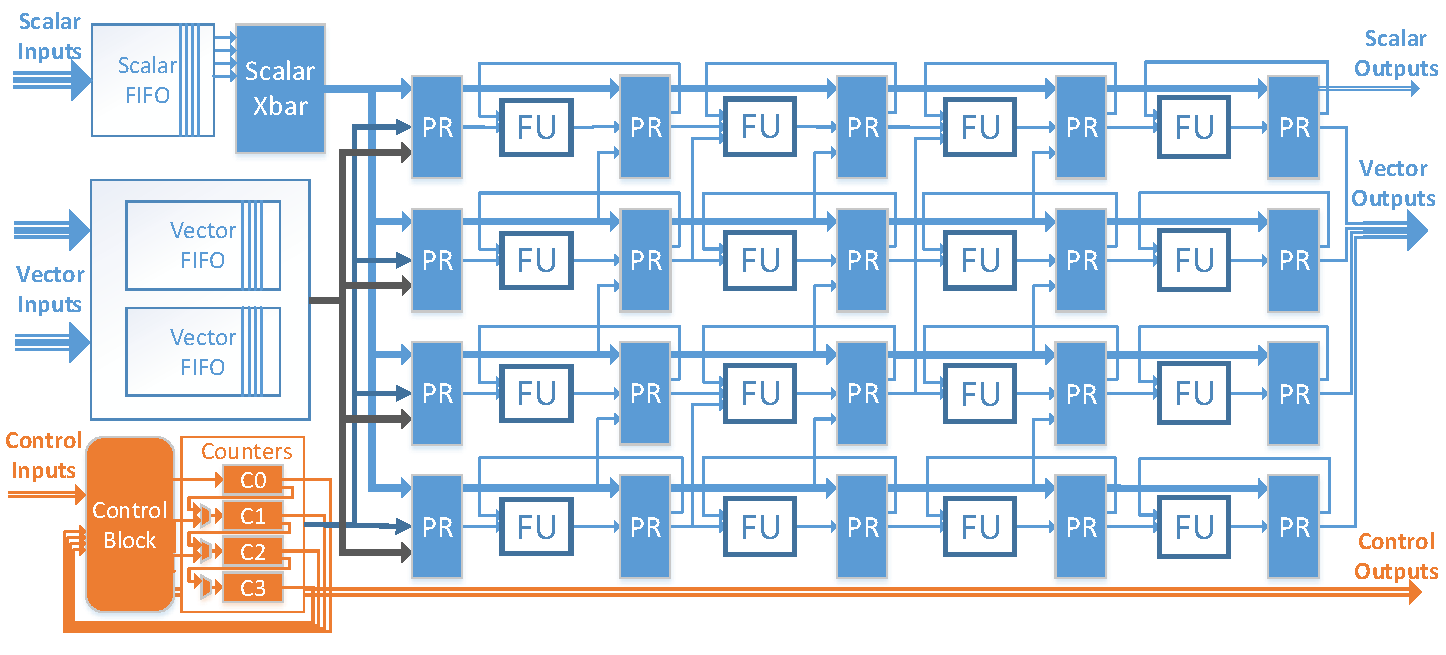
\includegraphics[width=0.82\textwidth]{figs/plasticineV2_simple.pdf}
  \vspace{-10pt}
  \caption{Pattern Compute Unit (PCU) architecture. We show only 4 stages and 4 SIMD lanes, and omit some control signals.
  \vspace{3pt}
}\label{fig:pcu}
\end{figure*}

\begin{figure*}[ht]
\centering
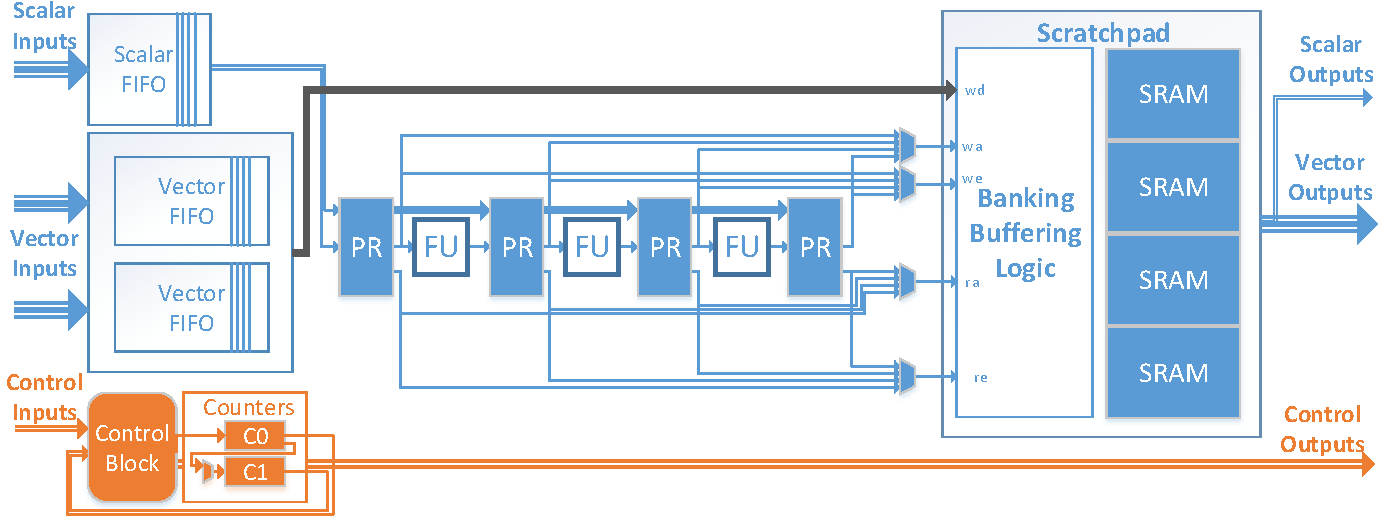
\includegraphics[width=0.82\textwidth]{figs/pmu.pdf}
  \vspace{-10pt}
  \caption{Pattern Memory Unit (PMU) architecture: configurable scratchpad, address calculation datapath, and control.}
  \label{fig:pmu}
  \vspace{3pt}
\end{figure*}

\begin{figure*}[ht]
\centering
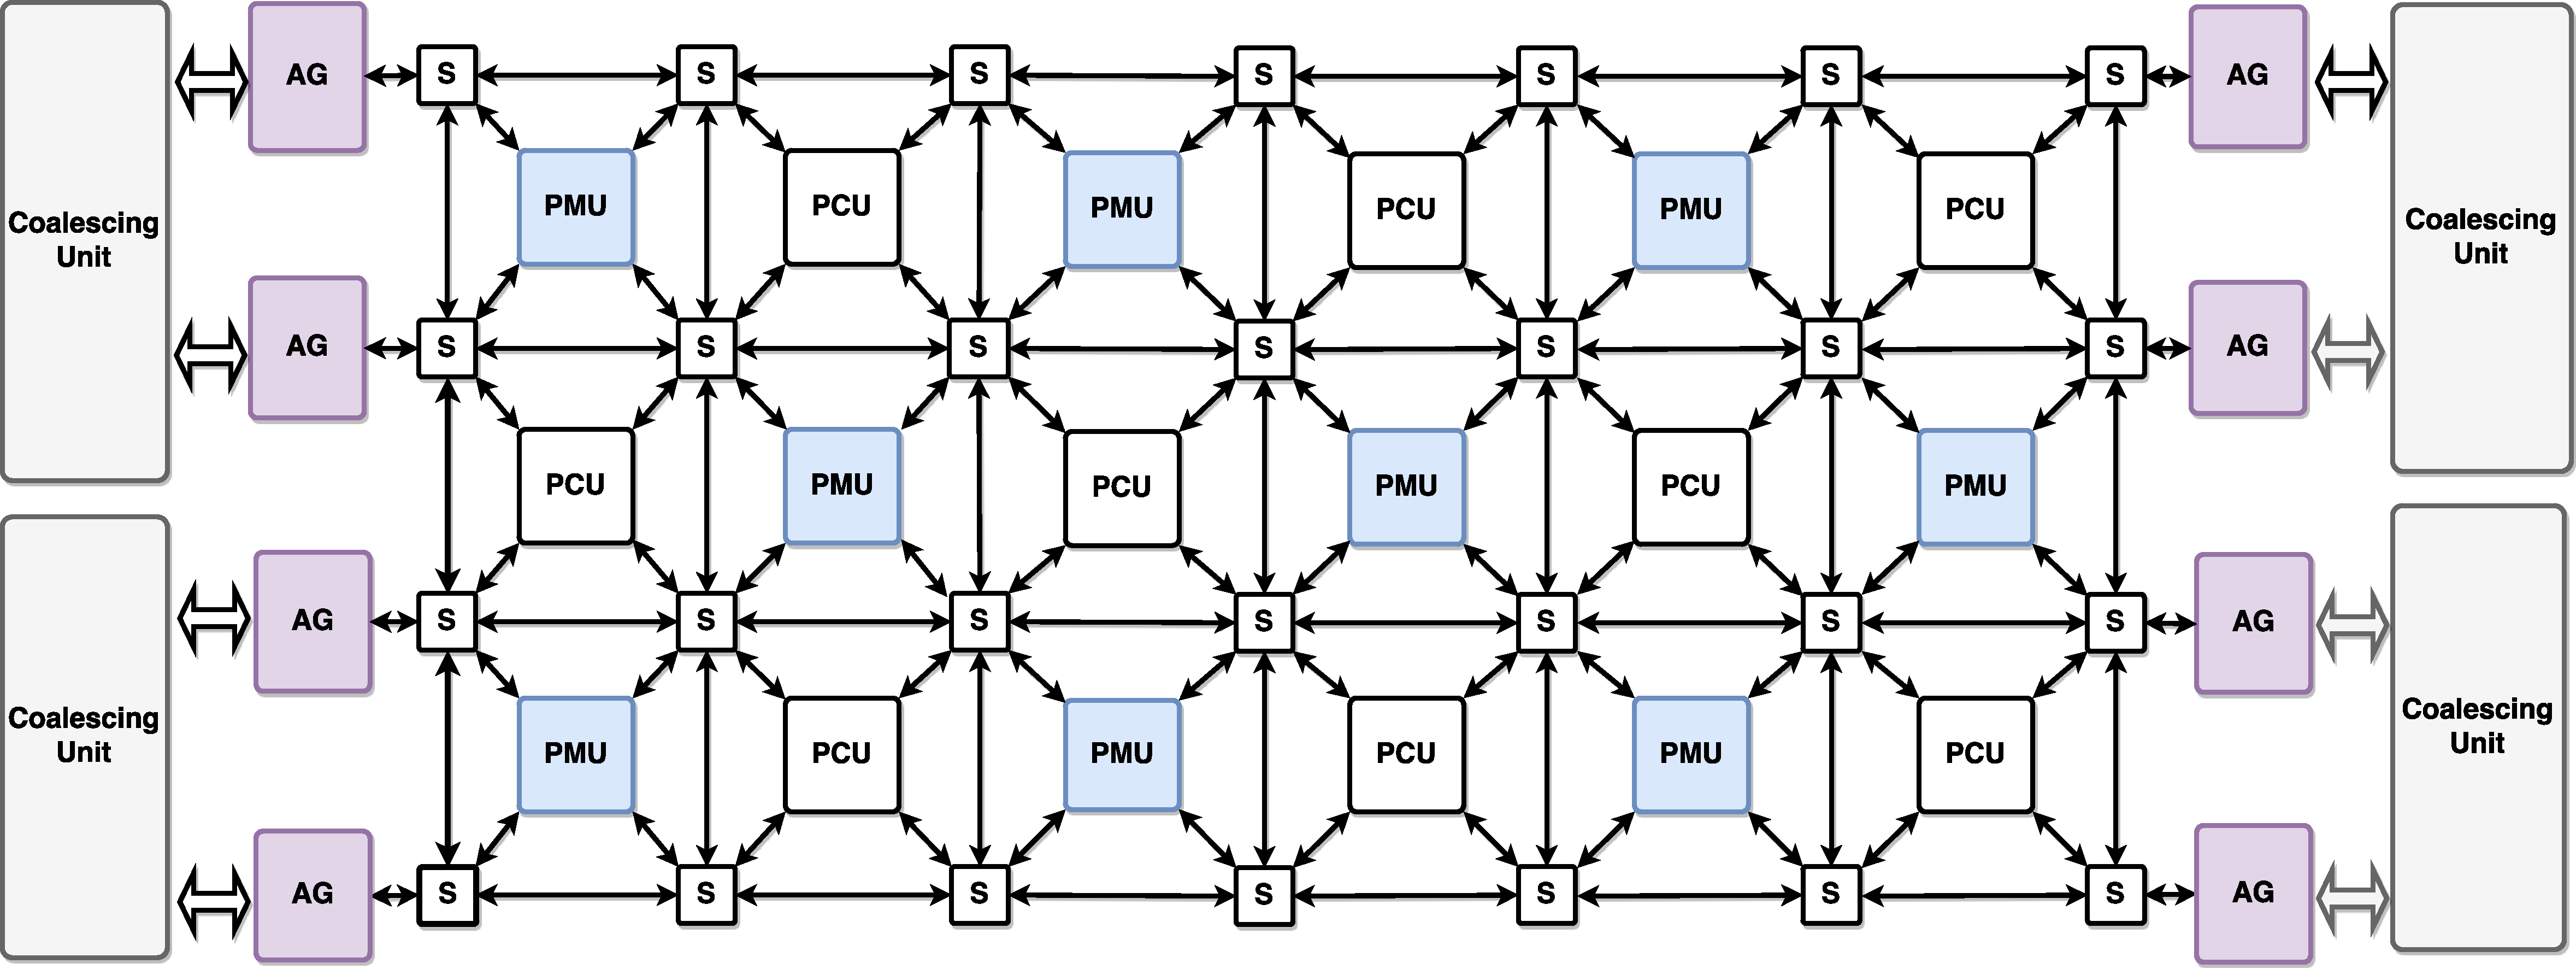
\includegraphics[width=0.9 \textwidth]{figs/network.pdf}
  \vspace{-10pt}
  \caption{Plasticine chip-level architecture (actual organization 16 x 8). All three networks have
  the same structure. \\
  PCU:Pattern Compute Unit, PMU: Pattern Memory Unit, AG: Address Generator, S: Switch Box.}
  \label{fig:interconnect}
  \vspace{0pt}
\end{figure*}
 %\vspace{-20pt}

\subsection{Pattern Compute Unit}
\label{ssec:PCU}
% \gist {Describe PCU datapath: Reconfigurable, pipelined SIMD stages, pipeline registers, counter chain.
% Describe connectivity between FUs: pipelined communication between stages, reduction tree across
% lanes, shift network between lanes. Control block consists of a few up-down counters and reconfigurable
% 'and' trees to co-ordinate with other PCUs.

% PCU and external world: PCU has 3 kinds of IO: scalar, vector, and control. Scalar and vector inputs
% are buffered using FIFOs at the input to decouple data producers and consumers.
% }

The PCU is designed to execute a single, innermost parallel pattern in
an application. As shown in Figure~\ref{fig:pcu}, the PCU datapath is organized as a multi-stage, reconfigurable SIMD pipeline.
This design enables each PCU to achieve high compute density, and exploit both loop-level
parallelism across lanes and pipeline parallelism across stages.

Each stage of each SIMD lane is composed of a \emph{functional unit} (FU) and associated pipeline registers
(PR). FUs perform
32 bit word-level arithmetic and binary operations, including support for floating point and integer operations. 
As the FUs in a single pipeline stage operate in SIMD, each stage requires only a single configuration register.
Results from each FU are written to its associated register. 
PRs in each lane are chained together across pipeline
stages to allow live values  propagate between stages within the
same lane. Cross-lane communication between FUs is captured using two types of intra-PCU networks: a reduction tree network that allows
reducing values from multiple lanes into a single scalar, and a shift network which allows using PRs as sliding windows
across stages to exploit reuse in stencil applications.
Both networks use dedicated registers within PRs to minimize hardware overhead.

PCUs interface with the global interconnect using three kinds of inputs and outputs (IO); scalar, vector, and control. Scalar IO is used to communicate
single words of data, such as the results of Folds. Each vector IO allows communicating one word per lane in the PCU, and is used in cases such as
reading and writing to scratchpads in PMUs and transmitting intermediate data across a long pipeline between multiple PCUs.
Each vector and scalar input is buffered using a small FIFO. Using input FIFOs decouples data producers and consumers, and simplifies inter-PCU control
logic by making it robust to input delay mismatches. Control IO is used to communicate control signals such as the start or end of execution of a PCU,
or to indicate backpressure.

A reconfigurable chain of counters generates pattern iteration
indices and control signals to coordinate execution. PCU execution begins when the control block enables one of the
counters. Based on the application's control and data dependencies, the control block can be configured to combine
multiple control signals from both local FIFOs and global control inputs to trigger PCU execution.
The control block is implemented using reconfigurable combinational logic and programmable up-down counters
for state machines.


\begin{figure*}[ht]
  \centering
  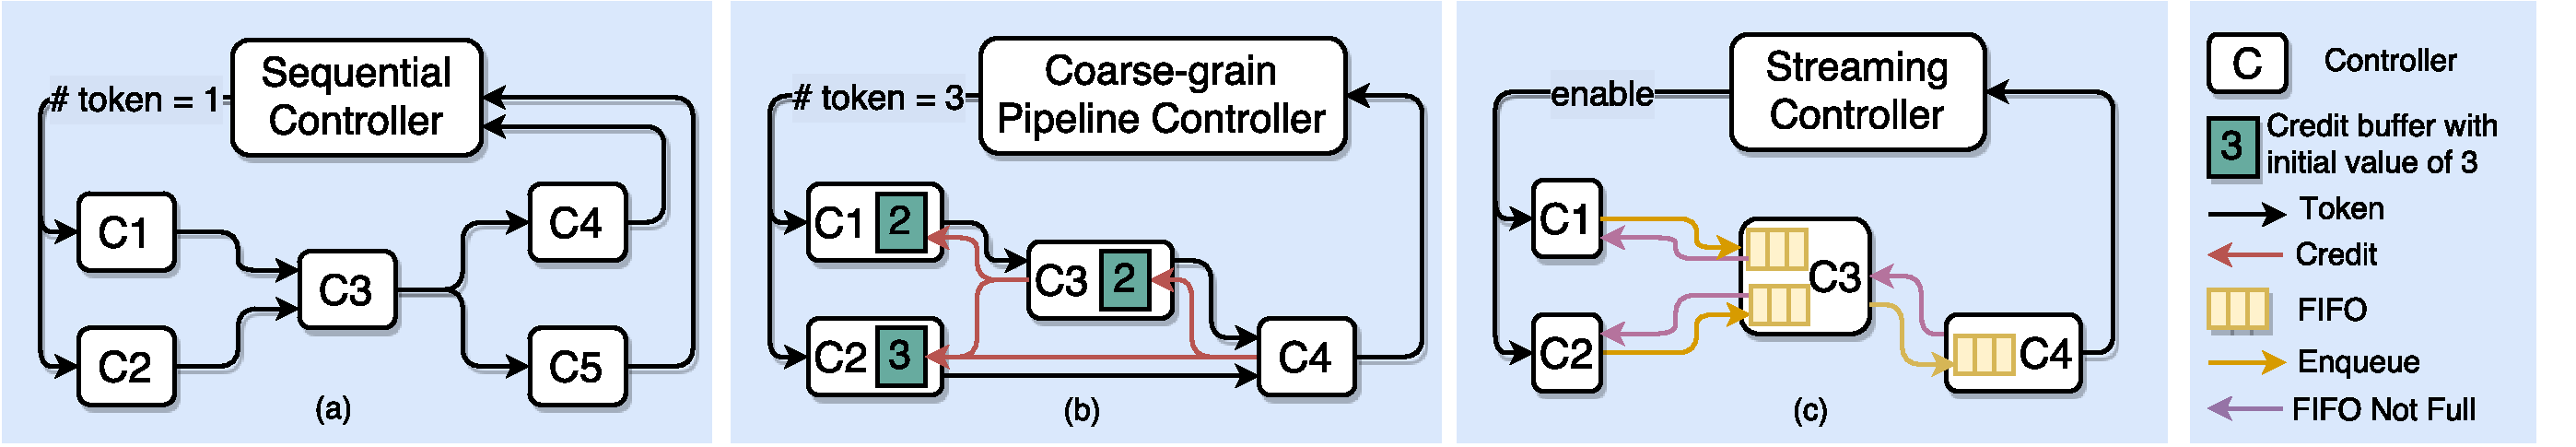
\includegraphics[width=1\textwidth]{figs/control.pdf}
  \vspace{-20pt}
  \caption{Sequential, coarse-grained pipelining, and streaming control schemes.}
  \label{fig:control}
\end{figure*}

%  Address Generators (AG) produce DRAM requests
%  into a coalescing unit, which arbitrates between AGs and coaleses requests to the same DRAM burst.
\subsection{Pattern Memory Unit}
\label{ssec:PMU}
% \gist{On-chip scratchpad with a reconfigurable integer pipeline.
%  FIFOs at inputs of PCUs and PMUs
% decouple PMU memory access from PCU execution. Scratchpad is banked with 16 banks,
% and can be configured in multiple modes to support various access patterns.
% Strided, N-buffered, FIFO, Line Buffer, Duplication etc.
% }
%For compute intensive applications, two factors need to be considered to both increase utilization and overall system energy efficiency. First, most memory accesses should be localized on the chip to decrease expensive DRAM accesses. Second, the architecture should include a memory hierarchy to lower the energy of repetitive accesses from ALUs~\cite{dark, LAP_TC12}.
%In Plasticine, memory hierarchy is supported in the form of PMUs distributed throughout the chip.
Figure~\ref{fig:pmu} shows the architecture of a PMU.
Each PMU contains a programmer-managed scratchpad memory coupled with a reconfigurable scalar datapath intended for address calculation.
As shown in Figure~\ref{fig:interconnect}, PMUs are used to distribute on-chip memory throughout the Plasticine architecture.
Plasticine makes a distinction between the operations involved in memory addresses calculation and the core computation
underlying applications. Address calculation is performed on the PMU datapath, while the core computation is performed within the PCU.
Several observations have motivated this design choice:
(i)  Address calculation involves simple scalar math, which requires simpler ALUs than the FUs in PCUs;
(ii) Using multiple lanes for address computation is often unnecessary for most on-chip access patterns; and
(iii) Performing address calculation within the PCU requires routing the addresses from the PCU to the PMU, which occupies PCU stages
     and output links, and can lead to PCU under-utilization.



The scratchpads are built with multiple SRAM banks matching the number of PCU lanes. Address decoding logic around the scratchpad
can be configured to operate in several banking modes to support various access patterns. \emph{Strided banking} mode supports
linear access patterns often found on dense data structures. \emph{FIFO} mode supports streaming accesses. \emph{Line buffer}
mode captures access patterns resembling a sliding window. \emph{Duplication} mode, where the contents are duplicated across all
memory banks, provides multiple read address channels to support parallelized on-chip gather operations.

Just as banking is important to feed multiple SIMD units to sustain compute throughput, \emph{N-buffering}, or generalized double buffering,
is just as important to support coarse-grained pipelines. The PMU scratchpad can be configured to operate as an N-buffer with any
of the banking modes described. N-buffers are implemented by partitioning the address space in each SRAM bank into N disjoint regions.
Using write and read state information, an appropriate offset is added to each bank's local address to access the correct data.

A programmable counter chain and control block triggers PMU execution similar to the PCU. Each PMU typically contains write address
calculation logic from the producer pattern, and read address calculation logic from the consumer pattern. Based on the state of
the local FIFOs and external control inputs, the control block can be configured to trigger the write address computation, read
address computation, or both, by enabling the appropriate counters.

\subsection{Interconnect}
\label{ssec:Interconnect}
Plasticine supports communication between PMUs, PCUs, and peripheral elements using
three kinds of interconnect - scalar, vector, and control. The networks differ in the granularity of
data being transferred; scalar networks operate at word-level granularity, vector networks operate at
multiple word-level granularity, and control networks operate at bit-level granularity. The topology
of all three networks is identical, and is shown in Figure~\ref{fig:interconnect}. All networks are
statically configured. Links in network switches include registers to avoid long wire delays.

Applications commonly contain nested pipelines, where the outer pipeline levels 
only require counters and some reconfigurable control. In addition, as outer pipeline logic
typically involves some level of control signal synchronization, they are control hotspots
which require a large number of control and scalar inputs and outputs. To handle outer pipeline logic in
an efficient manner, scalar and control switches share a reconfigurable control block and counters.
Incorporating control
logic within switches reduces routing to hotspots and increases PCU utilization.




\subsection{Off-chip Memory Access}
\label{ssec:Off-chip}
Off-chip DRAM is accessed from Plasticine using 4 DDR memory channels.
Each DRAM channel is accessed using several \emph{address generators} (AG) on two sides of the chip, as shown in Figure~\ref{fig:interconnect}.
Each AG contains a reconfigurable scalar datapath to generate DRAM requests, 
similar in structure to the PMU datapath shown in Figure~\ref{fig:pmu}. In addition, each AG contains FIFOs
to buffer outgoing commands, data, and incoming responses from DRAM. Multiple AGs connect to an address coalescing unit,
which arbitrates between the AGs and processes memory requests.

AGs can generate memory commands that are either \emph{dense} or \emph{sparse}. Dense requests are used to bulk transfer
contiguous DRAM regions, and are commonly used to read or write tiles of data. Dense requests are converted
to multiple DRAM burst requests by the coalescing unit. Sparse requests enqueue a stream of addresses into the coalescing
unit. The coalescing unit uses a coalescing cache to maintain metadata on issued DRAM requests and combines sparse
addresses that belong to the same DRAM request to minimize the number of issued DRAM requests. In other words, sparse memory loads trigger
a \emph{gather} operation in the coalescing unit, and sparse memory stores trigger a \emph{scatter} operation.



\subsection{Control Flow}
\label{ssec:Control}
%Plasticine uses a distributed \emph{token} and \emph{credit} based protocol to orchestrate control flow between PCUs and PMUs. 
%Tokens refer to feed-forward control flow signals, which are used to track the amount of data a PCU or PMU currently has available to operate on. Credits are signals which indicate back-pressure. They tell the PCU how many elements it can produce before its consumers will no longer be able to buffer its outputs. A unit can therefore execute when it has at least one token from all of its inputs, and one credit from all consumer units that it is writing to. 

%The architecture of the control block in each unit is shown in Figure~\ref{fig:controlBlock}.
%Both tokens and credits are implemented as 1-bit, single-cycle pulse control signals. 
%Each unit contains a set of configurable token buffers to track
%remaining tokens from each of its inputs.

%Figure~\ref{fig:ctrl} depicts the control logic configuration for three common outer loop control schemes: (a) \emph{sequential} execution, (b) \emph{coarse-grain pipelining}, and (c) \emph{streaming}. These control schemes correspond to outer loops in the input program, and determine how the execution of individual units are scheduled relative to other units. 
%In a sequential control flow, only one unit is active at any time.
%Therefore, when a parent controller receives a token, it will send
%a signal to initialize the first stage. 
%In coarse-grain pipelining, execution of stages is overlapped, the
%token buffer in each unit is initialized to the number of dependent pipeline stages. 
%Additionally, a credit buffer
%is allocated for any output the unit writes with an initialization of 2 to indicate double buffering at
%the consumer side. 
%Finally, in streaming, data
%dependencies between units are only enforced by states of FIFOs. In this scheme, a given unit is enabled to execute only if
%all of its input FIFOs are not empty, and all FIFOs it writes to are not full.

Plasticine uses a distributed and hierarchical control scheme that minimizes synchronization
between units in order to adapt to limited bit-wise connectivity in the interconnect. We support 
three types of controller protocols inferred from our high-level language constructs: (a) \emph{sequential} execution,
(b) \emph{coarse-grained pipelining}, and (c) \emph{streaming} (Figure~\ref{fig:control}).
These control schemes correspond to outer
loops in the input program, and determine how the execution of individual units are scheduled
relative to other units. Units are grouped into hierarchical sets of controllers. The control
scheme of sibling controllers is based on the scheme of their immediate parent controller.

In a sequential parent controller, only one data dependent child is active at any time.
This is commonly used when a program has loop-carried dependencies. To enforce data dependencies, we use
\emph{tokens}, which are feed-forward pulse signals routed through the control network. When the parent
controller is enabled, a single token is sent to all \emph{head} children with no data dependencies on their siblings. Upon
completing execution, each child then passes its token to consumers of its output data. Each
controller is enabled only when tokens from all dependent data sources are collected. 
Tokens from the last
set of controllers, whose data are not consumed by any sibling controller in the same level of hierarchy, are
sent back to the parent. The parent combines the tokens and either sends tokens back
to the heads for the next iteration, or passes the token along at its own hierarchy level when all
of its iterations have finished. 

In coarse-grained pipelines, child controllers 
are executed in a pipelined fashion. To allow concurrent execution, the parent controller sends \emph{N} \emph{tokens}
to the \emph{heads}, where \emph{N} is the number of data dependent children in the critical path. This
allows all children to be active in the steady state. To allow producers and consumers to work on
the same data across different iterations, each intermediate memory is \emph{M}-buffered, where \emph{M} is the
distance between the corresponding producer and consumer on their data dependency path. To prevent producers from
overflowing the down-stream buffer, each child controller handles backpressure by keeping
track of available down-stream buffer sizes using \emph{credits}.
The number of credits is statically initialized to M. Each producer decrements its credit count after producing
all the data for the ``current" iteration of the parent. Similarly, the consumer sends a credit back through the
network after consuming all the data for the ``current" iteration of the parent. 
In the coarse-grained pipelining scheme, each child is enabled when it has at least one token and one credit
available. 

Finally, child controllers with a \emph{streaming} parent controller
execute in a fine-grain pipelining fashion. This allows the compiler to fit a large inner pattern body by
concatenating multiple units to form a large pipeline. In streaming mode, children communicate
through FIFOs. A controller is enabled when all FIFOs it reads from are \emph{not
empty} and
all FIFOs it writes to are \emph{not full}. FIFOs are local to the consumer controller, so 
\emph{enqueue} and \emph{not empty} signals are routed from consumer to producer through the control network. 

To enforce these control protocols, we implement specialized reconfigurable control blocks using statically programmable counters,
state machines and combinational lookup tables. Each PCU, PMU, switch, and memory controller in the architecture has a control block. 
In general, controllers without any children are mapped to PCUs, while outer controllers are mapped to control logic in switches.
This mapping gives outer controllers, which often have many children to synchronize with, a higher radix for
communication. The hierarchy and distributed communication in Plasticine's control scheme allows the
compiler to leverage the multiple levels of parallelism available in nested parallel patterns with only minimum overhead from bit-level 
reconfigurability. 

%\emph{Up-down} counters in the control block track the number of tokens and credits from other units. 
%Each up-down counter provides 1-bit \emph{valid} and \emph{done} outputs, which signal when the counter is running and saturated, respectively. Look-up tables are used to combine valid signals and generate
%counter enable signals. 
%Done signals are similarly combined using look-up tables
%to generate one or more output tokens and/or credits. These control signals are sent out to other units using the control interconnect.

%Each PCU has an input control bus with several bits to carry input
%\emph{tokens}/\emph{credits}, and an output bus to carry several output
%\emph{tokens}/\emph{credits}. A main control block provides memory-mapped command
%and status registers to the host processor that manages execution of the entire Plasticine
%array. The main control block begins execution by generating a single
%token. Execution is completed when the token is returned to the main
%control block.

%\begin{figure}[ht]
%\centering
%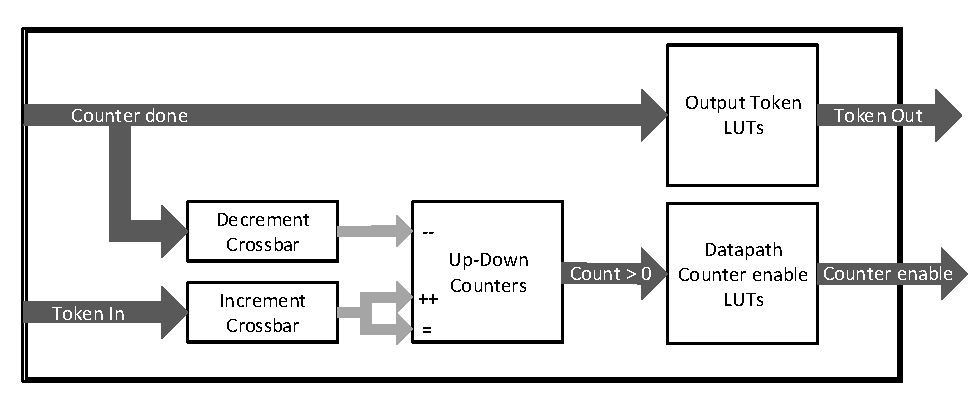
\includegraphics[width=0.45\textwidth]{figs/controlBlock.pdf}
%\caption{Control Block in a PCU.}
%\label{fig:controlBlock}
%\end{figure}

%\subsection{Memory Interfaces}
%\label{ssec:MemoryInterface}
%Several memory interfaces share a single physical DRAM channel. To optimize for
%the common case of off-chip address calculation, Plasticine has dedicated scalar
%compute units close to the memory interface.
%The PCU is designed to execute a single, potentially nested, loop of
%operations in an application. As shown in Figure~\ref{fig:cu}, the PCU
%is a multi-stage reconfigurable pipeline. Each pipeline stage includes
%a multi-lane functional unit and register set. This enables each PCU
%to achieve high compute density and exploit both loop-level
%parallelism across lanes and pipeline parallelism.  In
%Section~\ref{evaluation}, we evaluate PCUs with up to 32 stages and 4 to 32
%lanes.  Data locality is captured in each PCU using multiple
%scratchpad banks that can be statically configured to support various
%access patterns. A reconfigurable chain of counters generates of loop
%indices and control signals to coordinate execution. The counters are
%controlled by a control block, which implements the distributed
%control flow scheme for coarse-grained, task or pipeline parallel
%execution across multiple PCUs (see Section~\ref{ssec:controlflow}).
%
%
%{\bf Datapath:} The \emph{functional units} (FUs) can perform
%word-level (32b) arithmetic and logic operations. The FUs in a single
%pipeline stage operate in a SIMD, multi-lane fashion, hence requiring
%just one configuration register per stage. Each FU is associated with
%a set of pipeline registers -- denoted by the \emph{Regs} box in
%Figure~\ref{fig:cu} -- into which results from the FU are
%written. Registers in each lane are chained together across pipeline
%stages to allow live values to be propagated between stages in the
%pipeline.
%
%Table~\ref{t-cuPipeTypes} describes the different types of stages in
%each PCU. Stages are specialized in order to minimize area overheads
%without sacrificing flexibility. The first few stages in each PCU --
%like stages $0$ and $1$ in Figure~\ref{fig:cu} -- are
%\emph{read-write} stages and have maximum flexibility in choosing
%source and destination locations. \emph{Read-write} stages are
%followed by a number of \emph{regular} stages, such as Stage $2$ in
%Figure~\ref{fig:cu}, that can only consume data from previous
%stages. To support commonly occurring operations such as array
%accumulation, the last stage in each PCU is a \emph{write} stage that
%can write directly into the local scratchpads. The write address is
%obtained from a special pipeline register in the \emph{write}
%stage. \emph{Reduction} stages (Stage $3$ in Figure~\ref{fig:cu})
%implement a reduction tree across several stages to support scalar
%accumulations.
%

%
%
%\begin{table*}[]
%\centering
%\resizebox{\textwidth}{!}{%
%\begin{tabular}{@{}llll@{}}
%\bottomrule
%\textbf{Pipeline Stage Type} & \textbf{Source Locations}                                     & \textbf{Destination Locations}                          & \textbf{Inter-Lane Communication}   \\ \midrule
%Regular             & Previous Stage, Current Stage                         & Pipeline Registers                        & None                       \\ \midrule
%Read-Write          & Previous Stage, Current Stage, Scratchpads, Counters  & Pipeline Registers, Scratchpads           & None                       \\ \midrule
%Write               & Previous Stage, Current Stage                         & Pipeline Registers, Scratchpads           & None                       \\ \midrule
%Reduction           & Previous Stage, Current Stage                         & Pipeline Registers                        & Tree Network               \\ \midrule
%\end{tabular}
%}
%
%\caption{Types of PCU pipeline stages.}
%\label{t-cuPipeTypes}
%\end{table*}
%
%{\bf Scratchpad Banks:} Each local scratchpad has multiple memory
%banks to match the number of lanes in the datapath. Its capacity is in
%the few KBytes (2-32). A configurable address decoder provides a
%word-level addressing abstraction to the datapath and supports bank
%addressing schemes such as broadcast, round-robin, and strided
%modes. This allows for parallel accesses with random, sequential, and
%strided access patterns respectively. Each PCU can only read from its
%local scratchpads in the read-write pipeline stages. Scratchpads can
%be written either locally by write stages, or remotely from another
%PCU or a memory controller.
%
%{\bf Counter Chains:} Each PCU is equipped with a chain of
%reconfigurable counters to generate loop indices. Each counter can be
%configured with maximum and stride values, which can either be a
%constant or a value from one of the PCU input buses.  The counters can
%be linearly grouped into one or more chains to support
%multi-dimensional indexing found in perfectly nested loops.  For
%example, the counter chain shown in Figure~\ref{fig:cu} can be
%configured to operate as one 4-dimensional counter chain, two
%2-dimensional counter chains, or four independent counters.  Counter
%outputs are connected to the datapath as well as the scratchpad
%address ports to support linear addressing.
%
%Counters also act as the interface between data and control
%paths. Each counter can be individually managed by an `enable'
%signal. When the counter wraps around, a one-cycle `done' pulse is
%generated. The control block in each PCU generates the `enable'
%signals and uses the `done' signals to track and handle inter-PCU
%control flow.
%

%
%\subsection{Inter-PCU Interconnect}
%
%The data interconnect operates at a granularity of a vector of 16 32-bit words, or 512 bits. The control interconnect operates at a bit-level
%  granularity.
%
%Figure~\ref{fig:interconnect} shows the static interconnection topology between PCUs.
%PCUs are laid out as a two-dimensional array in a static hybrid interconnection network.
%Plasticine uses separate interconnection networks for the data path and
%control path. The data interconnect routes data at the granularity of a vector of 16
%32-bit words, or 512 bits. The control interconnect uses a bit-level interconnect to provide greater flexibility
%to route control signals between PCUs. Both interconnects have registers in the switches
%to avoid long critical paths and sustain a high clock rate.
%
%Main memory is accessed on the left and right columns of the array through reconfigurable
%memory command generators, as shown in figure~\ref{fig:interconnect}. The memory command
%generators can be configured to either operate in burst mode to optimize loading dense
%data structures, or scatter-gather mode to optimize loading sparse data structures. In
%scatter-gather mode, memory command generators support address coalescing to minimize
%off-chip DRAM access.
%
%
\subsection{Application Mapping}
\label{mapping}
We begin with an application represented as a hierarchy of parallelizable dataflow pipelines written in a parallel pattern-based language called
the Delite Hardware Definition Language (DHDL)~\cite{dhdl}.
Prior work~\cite{delite2maxj} has shown how applications expressed in the parallel patterns described in Section~\ref{patterns}
can be automatically decomposed into pipelines in DHDL.
Pipelines in DHDL are either \emph{outer controllers} which contain only other pipelines, or \emph{inner controllers} which contain no other controllers, only dataflow graphs of compute and memory operations.

To map DHDL to Plasticine, we first unroll outer pipelines using user-specified or auto-tuned parallelization factors.
The resulting unrolled representation is then used to allocate and schedule \emph{virtual} PMUs and PCUs.
These virtual units are an abstracted representation of the units in Plasticine which have an infinite number of available
inputs, outputs, registers, compute stages, and counter chains.
As outer controllers contain no computation, only control logic, they map to a virtual PCU with no compute stages, only control logic and counter chains.
The computation in inner controllers is scheduled by linearizing the data flow graph and mapping the resulting list of operations
to virtual stages and registers.
Each local memory maps to a virtual PMU. Stages used to compute read and write addresses for this memory are copied to the virtual PMUs.

We then map each virtual unit into a set of physical units by partitioning its stages.
Virtual PCUs are partitioned into multiple PCUs, while PMUs become one PMU with zero or more supporting PCUs.
While graph partitioning is NP-hard in general, each virtual unit tends to have far less than 200 compute stages with very few cyclic dependencies.
This means that a greedy algorithm with a few simple heuristics can reasonably approximate a perfect physical unit partitioning.
In our partitioning algorithm, we use a cost metric which calculates the number of physical stages, live variables per stage, and scalar and vector input/output buses required for a given partitioning.
Note that these communication and computation costs are always statically predictable because we begin with a full dataflow representation of the application.
Using our heuristics, the compiler selects a proposed partitioning
where all PCUs and PMUs are physically realizable given some chosen set of
Plasticine architecture parameters (number of PCUs, PMUs, stages, lanes, buses, etc.) and which maximize the ALU and local memory utilization.

Following partitioning, we generate the control logic corresponding to the controller hierarchy
as described in Section~\ref{ssec:Control}. We then perform hierarchical binding of virtual hardware nodes to physical hardware
resources, including datapath and control path placement and routing, register allocation of SIMD
units, including mapping stages to physical ALUs, and allocating scratchpads and control resources. The hierarchical nature of Plasticine allows us to
dramatically reduce the search space with less than 1000 nodes in each level of mapping.

Given this placement and routing information, we then generate a Plasticine configuration description, akin to an assembly language, which is
used to generate a static configuration ``bitstream'' for the architecture.
The hierarchical architecture, coupled with the coarse granularity of buses between compute units, allows our entire
compilation process to finish (or fail) in only a few minutes, as compared to the hours it can take to generate FPGA configurations.

\begin{figure*}
\centering

\begin{tabular}{p{0.01cm} p{4.6cm} p{0.01cm} p{4.6cm} p{0.01cm} p{4.6cm} p{0.9cm}}
%%% trim = right, bottom, left, top
\textbf{a.} & {\includegraphics[clip, trim=0.4cm 3.3cm 1.0cm 1.2cm, width=4.6cm]{figs/Stages.pdf}} &
\textbf{b.} & {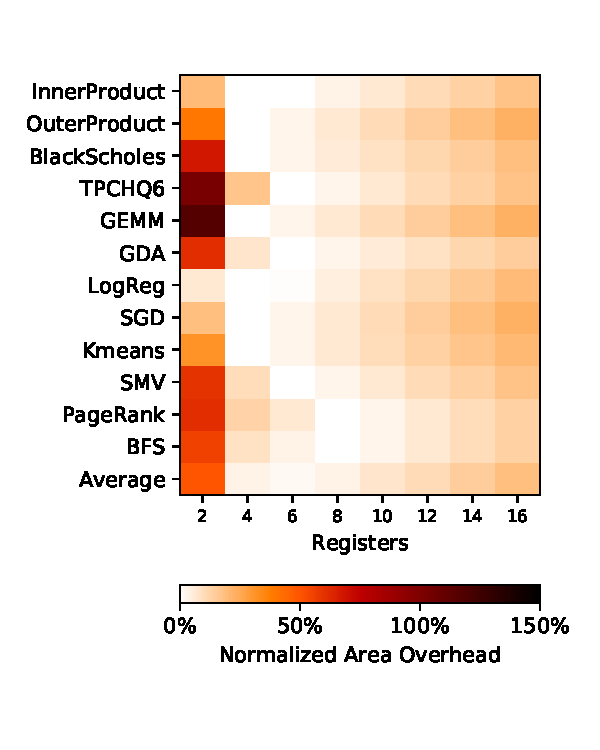
\includegraphics[clip, trim=0.4cm 3.31cm 1.0cm 1.2cm, width=4.6cm]{figs/Registers.pdf}} &
\textbf{c.} & {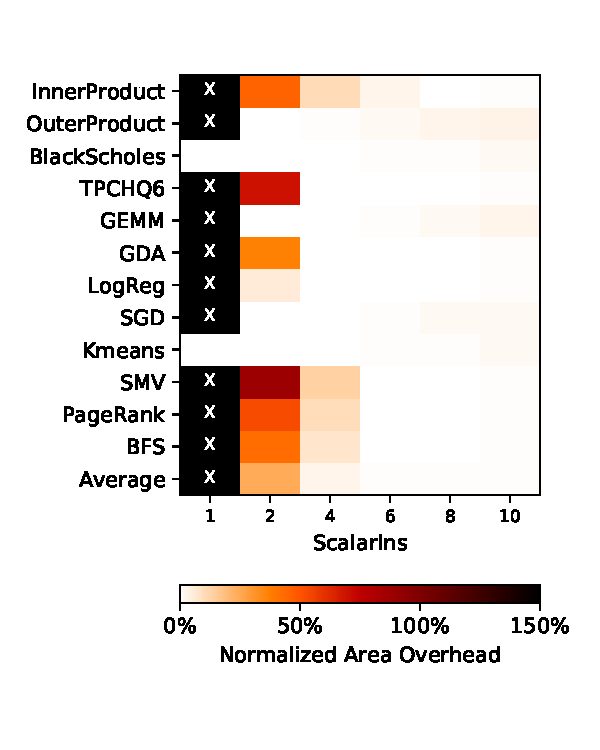
\includegraphics[clip, trim=0.4cm 3.31cm 1.0cm 1.2cm, width=4.6cm]{figs/ScalarIns.pdf}} &
{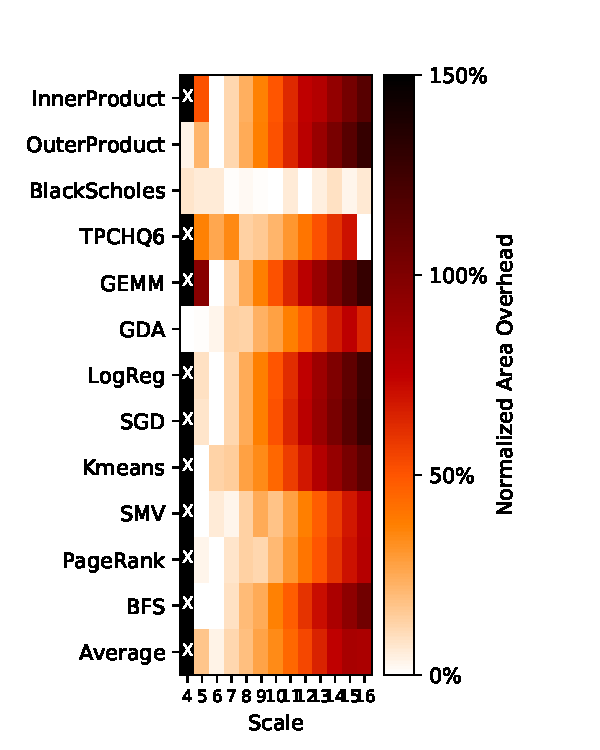
\includegraphics[clip, trim=6.4cm 0.4cm 0.4cm 0.4cm, height=4.6cm]{figs/Scale.pdf}} \\
 

\textbf{d.} & {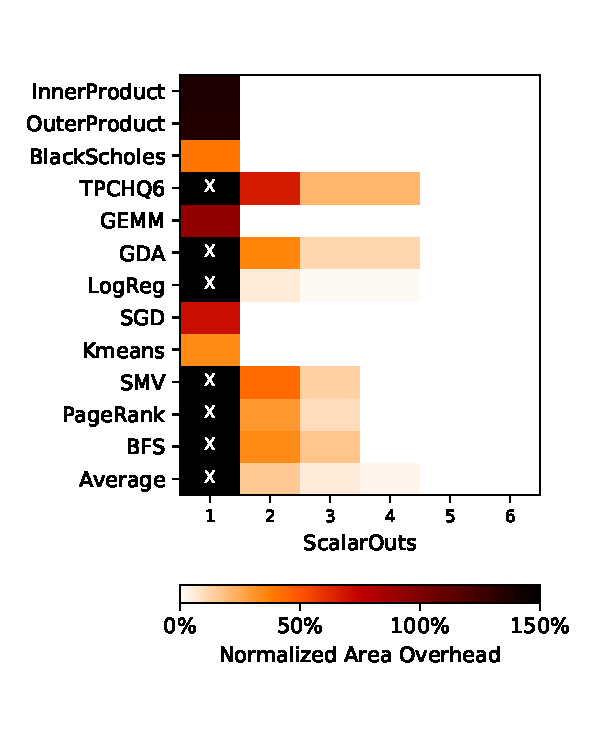
\includegraphics[clip, trim=0.4cm 3.31cm 1.0cm 1.2cm, width=4.6cm]{figs/ScalarOuts.pdf}} &
\textbf{e.} & {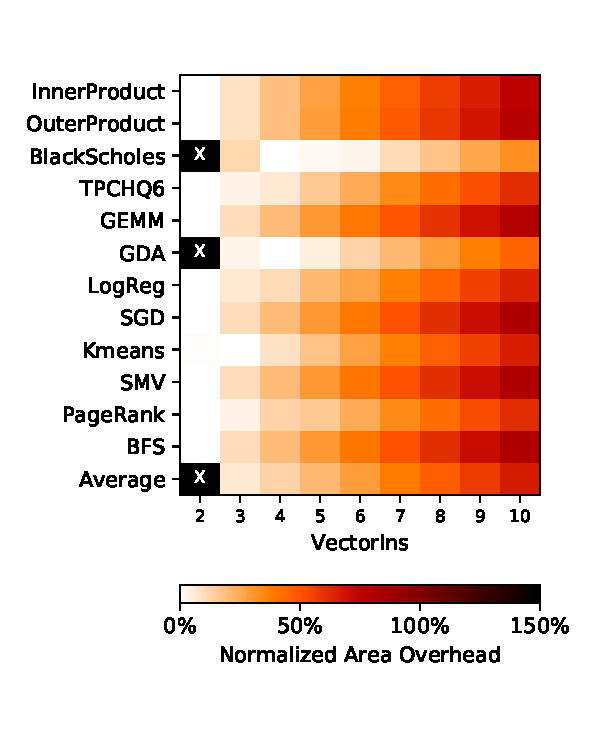
\includegraphics[clip, trim=0.4cm 3.31cm 1.0cm 1.2cm, width=4.6cm]{figs/VectorIns.pdf}} &
\textbf{f.} & {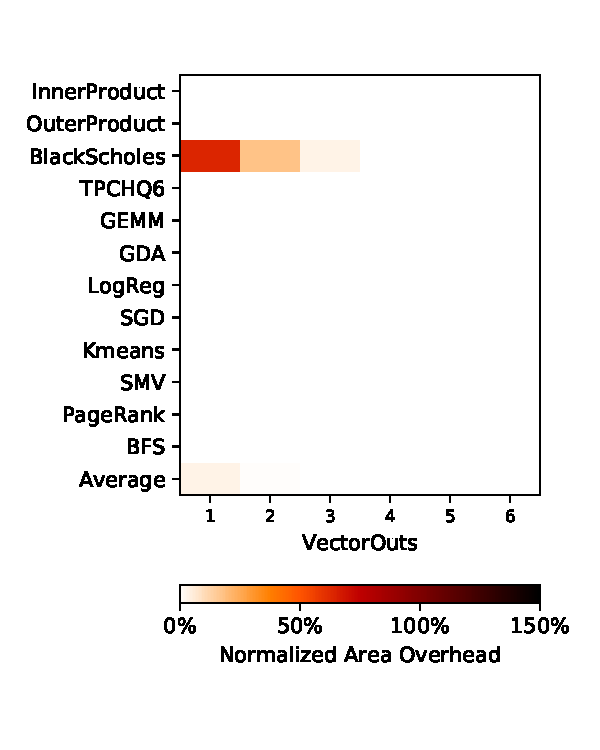
\includegraphics[clip, trim=0.4cm 3.31cm 1.0cm 1.2cm, width=4.6cm]{figs/VectorOuts.pdf}} &
{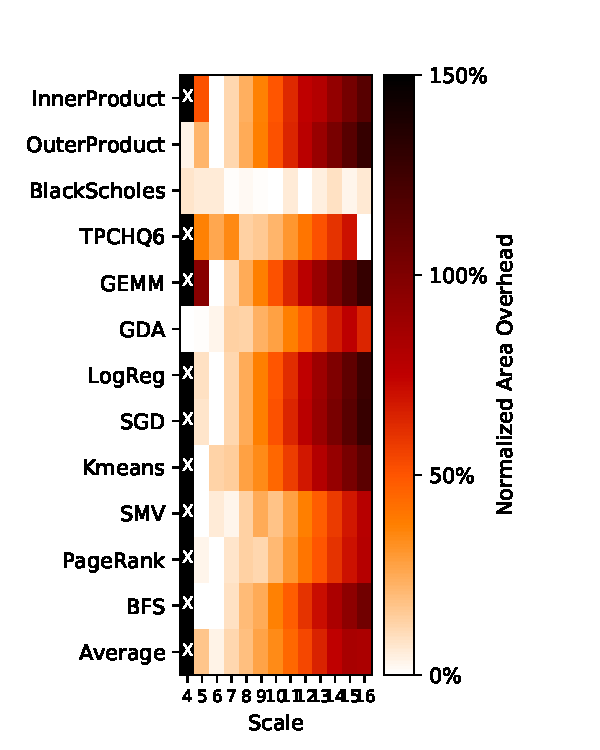
\includegraphics[clip, trim=6.4cm 0.4cm 0.4cm 0.4cm, height=4.6cm]{figs/Scale.pdf}} \\

\end{tabular}
\vspace{-10pt}
\caption{Area overhead ($Area_{PCU}/Min_{PCU} - 1$) while sweeping various Plasticine PCU parameters for a subset of our benchmarks. $Min_{PCU}$ is benchmark-specific minimum possible area. Areas marked with an $\times$ denote invalid parameters for the given application. \emph{a.}~Stages per PCU; \emph{b.}~Registers per FU with 6 stages; \emph{c.}~Scalar~inputs~per~PCU with 6 stages and 6 registers; 
\emph{d.}~Scalar~outputs~per~PCU with 6 stages, 6 registers, and 6 scalar inputs; \emph{e.}~Vector~inputs~per~PCU with 6 stages and 6 registers; and \emph{f.}~Vector~outputs~per~PCU with 6 stages, 6 registers, and 3 vector inputs. }
\label{fig:sizing}
\end{figure*}

\subsection{Architecture Sizing}
\label{sizing_section}

	%                   & \multicolumn{3}{c}{\textbf{Pattern Memory Unit}}  \\ \midrule
	%                   & \multicolumn{3}{c}{\textbf{Pattern Compute Unit}} \\ \midrule
	%                   & \multicolumn{3}{c}{\textbf{Architecture}}         \\ \midrule
\begin{table}[]
\centering
\resizebox{\columnwidth}{!}{%
\begin{tabular}{llcc}
\toprule
	                    & \textbf{Component}      & \textbf{Range}             & \textbf{Final Value} \\ \midrule
	                    & Lanes                   & 4, 8, 16, 32               & 16                   \\
	                    & Stages                  & 1 -- 16                    & 6                    \\
	\textbf{Pattern}    & Registers/Stage         & 2 -- 16                    & 6                    \\
	\textbf{Compute}    & Scalar Inputs           & 1 -- 16                    & 6                    \\
	\textbf{Unit}       & Scalar Outputs          & 1 -- 6                     & 5                    \\
	                    & Vector Inputs           & 1 -- 10                    & 3                    \\
	                    & Vector Outputs          & 1 -- 6                     & 3                    \\ \midrule
	                    & Bank Size               & 4, 8, 16, 32, 64KB         & 16KB                  \\
	                    & \emph{Scratchpad Banks} & \emph{Number of PCU Lanes} & 16                   \\
	                    & \emph{Total Scratchpad} & \emph{Bank size * banks}   & 256KB                \\
	                    & Stages                  & 1 -- 16                    & 4                    \\
	\textbf{Pattern}    & Registers/Stage         & 2 -- 16                    & 6                    \\
	\textbf{Memory}     & Scalar Inputs           & 1 -- 16                    & 4                    \\
	\textbf{Unit}       & Scalar Outputs          & 0 -- 6                     & 0                    \\
	                    & Vector Inputs           & 1 -- 10                    & 3                    \\
	                    & Vector Outputs          & 1 -- 6                     & 1                    \\ \midrule
\textbf{Architecture} & PCUs                    & ---                        & 64                   \\
	                    & PMUs                    & ---                        & 64                   \\
\bottomrule
\end{tabular}
}
\caption{Design space and final selected parameters.}
\label{t-parameters}
\vspace{-20pt}
\end{table}


%Note that in this study, we assume all PCUs and PMUs are homogeneous, i.e. we do not investagate architectures with a mix of PCU or PMU designs.
Thus far, we have described a parameterized architecture composed of, among other things, PCUs, PMUs, and interconnect.
We now describe our process for tuning the PCU and PMU parameters to create the final Plasticine architecture that we evaluate in Section~\ref{evaluation}.
Table~\ref{t-parameters} summarizes the architecture parameters under consideration, the possible values for each, and the final value we selected.
To improve the probability of application routability, we restrict PMUs and PCUs to be homogeneous across the architecture. 

In selecting design parameters, we first prune the space by analyzing the characteristics of the benchmarks listed in Table~\ref{t-apps}.
Based on models of the performance of each benchmark, we determine that the ideal inner controller parallelization factor across all benchmarks is between 8 and 32.
In Plasticine, this corresponds to Pattern Compute Units with between 8 and 32 SIMD lanes.
We select a balanced architecture with 16 lanes. Vectors of 16, 4 byte words also conveniently match our main memory's burst size of 64 bytes.
For the PMU scratchpads, we found that ideal tile sizes for our benchmarks are at most 4000 words per bank.
We therefore set the PMU to have 16 configurable, 16KB banks, for a total of 256KB~per~PMU.

We next search the remaining architectural space to select the number of stages, registers per stage, inputs, and outputs per PCU.
In our programming model, parallelizing outer controllers corresponds in hardware to duplicating inner controllers.
This means that we can assume that, to a first order, outer loop parallelization in a given application will not change its ideal
PCU parameters, only the required number of PCUs. We therefore fix each benchmark with realistic parallelization factors and use
these benchmarks to determine how to minimize the total PCU area while maximizing useful compute capacity.
Note that we must also allow the number of required PCUs to vary, as these parameters directly impact how many physical PCUs a virtual PCU will require.
Given the minimized PCU design, we can then create a Plasticine architecture with maximum performance for a given total chip area budget.




% Since the computation requirements do not change with outer control parallelization, we can assume 
% In this study, we set each benchmark to some realistic, fixed parallelization factors and allow the number of PCUs to vary.
% We then tune the parameters to minimize total required PCU area. To a first order, parallelizing outer control structures only changes the
% In the common case where pipeline drainage times are only a minor percentage of total runtime, these PCU parameters have little direct impact on application performance.
% Instead, they impact total chip area and accelerator utilization. However, while unused components can be clock-gated to save power, 
% underutilized areas of the chip would be better spent
We use a model-driven, brute force search to tune each architectural parameter across different applications.
To drive this search, we use benchmark-normalized \emph{area overhead} as a cost metric for useful PCU area.
When tuning a parameter, we sweep its value. For each proposed value, we sweep the remaining space to find the minimum possible PCU Area ($Area_{PCU}$).
We then normalize these areas based on their minimum ($Min_{PCU}$) and report the overhead of each possible parameter value as $Area_{PCU}/Min_{PCU} - 1$.
The area of a single PCU is modeled as the sum of the area of its control box, FUs, pipeline
registers, input FIFOs, and output crossbars.
The total number of PCUs required for a given set of design parameters is calculated using the mapping procedure outlined in Section~\ref{mapping}. 

In our studies, we found that the ordering of parameters during tuning made little difference to the final architectural design. 
For simplicity, we report a search procedure using one possible ordering, but any ordering would result in the same final parameter values.

%We search this space by isolating the effects of
%We present a simplified version of our procedure for searching this space.
We first examine the space defined by the number of stages per physical PCU.
All other parameters are left unrestricted.
Figure~\ref{fig:sizing}a shows the estimated area overheads after sweeping the number of stages between 4 and 16.
Here, we see that the ideal number of stages per PCU is 5 or 6 for most benchmarks.
In these benchmarks, the amount of compute per pattern is fairly small, allowing patterns to be mapped to a single PCU.
At least 5 stages are required for a full cross-lane reduction tree within the PCU.
In BlackScholes, the core compute pipeline has around 80 stages. This is long enough that stages per PCU has little impact on average FU utilization.
In TPCHQ6, the core computation is 16 stages long, meaning the area overhead is minimized at 8 and 16 stages (even divisors of the compute).
We select 6 stages per PCU as a balanced architecture across all of our benchmarks. 
This choice means that applications like TPCHQ6 with a relatively small number of operations that does not 
divide evenly by 6 will underutilize PCU partitions, but this is an inevitable consequence of partitioning over homogeneous units.

%\begin{table}[]
%\centering
%\resizebox{\columnwidth}{!}{
%\begin{tabular}{@{}llll@{}}
%\bottomrule
%\textbf{Benchmark} & \textbf{Description}                                                  & \textbf{Data Size(s)}                          & \textbf{Data Type} \\ \midrule
%Inner Product      & Vector inner product                                                  & 768,000,000                                    & float32       \\ \midrule
%Outer Product      & Vector outer product                                                  & 76,800 $\times$ 76,800                         & float32       \\ \midrule
%Black-Scholes      & Floating-point financial analysis                                     & 96,000,000 entries                             & float32       \\ \midrule
	%TPC-H Query 6    & \shortstack[l]{ Database query benchmark \\with filter-reduce}        & 960,000,000 entries                            & int32     \\ \midrule
	%GEMM             & \shortstack[l]{Tiled general matrix multiplication}                   & 47 $\times$ 7,680 * 7,680 $\times$ 3,840       & float32       \\ \midrule
%GDA                & \shortstack[l]{Generalized Discriminant Analysis}                     & 3,840,000 points; 96 dims                      & float32       \\ \midrule
	%LogReg           & \shortstack[l]{Iterative Logistic Regression}                         & 5 iters; 1,536 points; 384 dims                & float32       \\ \midrule
	%SGD              & \shortstack[l]{Iterative Stochastic Gradient\\ Descent}               & 30 iters; 38,400 points; 768 dims              & float32       \\ \midrule
	%Kmeans           & \shortstack[l]{Iteratively groups points by \\nearest of K centroids} & 50 iters; 1,536 points; 96 dims; K = 20        & float32       \\ \midrule
	%CNN              & \shortstack[l]{Convolutional Neural Network \\inference}              & model size 147456, data size 393216            & float32       \\ \midrule
	%SMDV             & \shortstack[l]{Sparse Matrix Dense Vector \\multiplication}           & 3,840 $\times$ 3,840 with $E[NNZ]_{node} = 60$ & float32       \\ \midrule
	%PageRank         & \shortstack[l]{Iteratively ranks nodes based \\on incoming edges}     & 100 iters; 7,680 pages                         & int32     \\ \midrule
	%BFS              & \shortstack[l]{Breadth-First Search \\calculating all node depths}    & $E[edges]_{node} = 8$ $\times$ 10 layers       & int32     \\ \midrule
%\end{tabular}
%}
%\caption{Evaluation benchmarks.}
%\label{t-apps}
%\vspace{-20pt}
%\end{table}


We next determine the number of registers per FU. We again sweep the parameter space, fixing the number of stages at 6 but leaving all other parameters unrestricted. 
From Figure~\ref{fig:sizing}b, we see that the ideal number of registers across most applications is between 4 and 6.
This directly corresponds to the maximum number of live values at any given point in each PCU's pipeline of stages.
Below 4 registers, PCUs are constrained by the number of live values they can hold at a given time, causing extraneous partitioning. Above 8 registers per FU,
the cost of the unused registers becomes noticeable relative to the total PCU area.
We select 6 registers per FU.

Following the same procedure, we determine the number of scalar inputs and outputs. Scalar logic is relatively cheap, but, like registers, lack of available scalar 
inputs or outputs can cause logic to be split across many PCUs, creating large overheads from unutilized logic. 
Thus, we see in Figure~\ref{fig:sizing}(c,d) that each benchmark has some minimum number of inputs and outputs required, after 
which adding more of either has little impact. 
We select 6 scalar inputs and 5 scalar outputs, as this minimizes area overhead across all benchmarks.


Finally, we tune the vector inputs and outputs per PCU in the same manner. Vectors are tuned separately from scalars, as the two use different interconnect paths between
PCUs and different registers within PCUs. Note here that vector inputs are associated with input FIFOs, which represent a sizeable fraction
of PCU area. We therefore want to minimize vector inputs as much as possible. However, as seen in Figure~\ref{fig:sizing}e, due to limitations in splitting across PCUs, 
BlackScholes and GDA are restricted to having at least 3 vector inputs.
Figure~\ref{fig:sizing}f shows that vector outputs are relatively inexpensive and have little impact on required design area. 
We thus choose 3 vector inputs and 3 vector outputs per PCU.

Using a similar approach, we also select the PMU parameters given in Table~\ref{t-parameters}. Note that the number of 
vector inputs and outputs for PMUs trivially correspond to the read, write, and data buses of the scratchpad. 
PMUs currently never use scalar outputs, as the compiler always maps the results of memory reads to vector buses.

After this tuning process, we now have a 
tuned PCU and PMU design. Based on profiling of each benchmark, we choose 16~$\times$~8 units.
We also experimented with multiple ratios of PMUs to PCUs. 
We choose a 1:1 ratio of PMUs to PCUs. 
While larger ratios (e.g. 2:1 PMUs to PCUs) improved unit utilization on some benchmarks, these ratios were less energy efficient.
% Next, we determine the number of vector inputs available per PCU. We fix the number of stages at 6 but leave the number of outputs unrestricted.
% For this experiment, we also account for switchbox area as a function of the number of buses to be switched, assuming one switchbox required per PCU on average.
% Figure~\ref{fig:sizing}e shows the results of sweeping the number of inputs between 1 and 8 on the same benchmarks.
% We can see from this figure that the ideal number of inputs for all benchmarks is 3 or 4. Below 3, the cost of underutilized PCUs dominates.
% Above 4, the area per operation slowly increases due to increasing switchbox and control sizes while the number of required PCUs remains unchanged.
% We select 4 vector inputs per PCU, as this gives near minimal area per operation cost across all of our benchmarks.


% Finally, we sweep the space of output vectors per PCU between 1 and 8, again modeling the total area as the sum of switchboxes and simplified PCUs.
% Figure~\ref{fig:sizing}f gives the normalized area per operation across the same subset of benchmarks.
% From this figure, we see that the ideal number of output vectors per compute unit is between 2 and 5, depending on the benchmark.
% We select 4 output vectors per PCU, as this gives a balanced design across all benchmarks.




%Additionally, communication between two pipelines typically take place
% via scratchpads, (ii) Pipelines are often imperfectly nested in multiple levels,
% requiring a general method to handle iterators of imperfectly nested outer pipelines.
% Plasticine handles these issues using an distributed execution model by favoring duplication over communication,
% as detailed below:
% \begin{itemize}
%   \item Inter-PCU communication via scratchpads: Writing to a remote scratchpad requires transferring
%     both write addresses and data through the interconnect. As each PCU is vectorized, this requires
%     a lot of interconnect bandwidth and would hence lead to power and area inefficiencies.
%     Plasticine performs write address calculation at the destination PCU. This requires only the data to be
%     passed through the interconnect. To facilitate this, counter chains at the source PCU are duplicated
%     at the destination, and the \emph{read-write} pipeline stages in the destination PCU are used to
%     compute the write address. Tokens that begin execution at the source PCU are routed to the destination
%     PCU as well. These tokens start the duplicated source PCU counters at the destination after a statically
%     determined delay, to offset the latency in data arrival and write address calculation.

%   \item Counter chains of imperfectly nested outer pipelines: Counter chains of outer pipelines are duplicated
%     in the PCUs corresponding to each of its inner pipelines that use the outer counters in the datapath. The
%     outer counters are updated in a distributed fashion when each inner PCU finishes execution by chaining the
%     inner counters with the outer counters.
% \end{itemize}

% \christos{need an example here}

% \subsection{PISA}
% Plasticine exposes a programming interface called Plasticine ISA (PISA). PISA is specified textually using a JSON-based
% format, which is parsed and assembled into a configuration bitstream.
